\section{Desenvolvimento realizado na empresa}
\label{sec:desenvolvimento}

{Nesta sessão será apresentada a ferramenta desenvolvida como solução ao problema de acessibilidade em  \textit{e-commerce} da organização, abordando as técnicas e tecnologias utilizadas e contribuições para a empresa.}

\subsection{A problemática e a solução proposta}

{A problemática tratava-se de transformar um \textit{e-commerce} legado sem práticas de acessibilidade em um \textit{e-commerce} acessível e bem construído focando em dar suporte e eliminar barreiras de acesso que as pessoas com deficiências visuais apresentam ao acessar um sistema como esse. Como requisitos principais para a solução ser aceita tínhamos que construir ou adaptar os componentes incluindo práticas de acessibilidade, dar suporte a diversos tipos de navegações que o usuário pudesse escolher, construir uma painel administrativo onde apresentasse um \textit{dashboard} com gráficos acessíveis para o acompanhamento das vendas.

Para tratar essa problemática foi necessário dividi-la em pequenas fases e trabalhar isoladamente em cada uma delas, visto que essas fases dependiam uma da outra e elas foram desenvolvidas de forma cronológica partindo de pesquisas à testes. 

No total foram preciso quatro fases, sendo a primeira fase voltada para o entendimento do problema e do uso das novas tecnologias como também entender as limitações do projeto. A segunda fase estava voltada na construção e adaptação da interface do usuário seguindo tudo o que foi levantado na fase de entendimento do problema. A terceira fase teve foco na construção do painel administrativo e no \textit{dashboard}, além do planejamento de componentes e na construção de gráficos acessíveis. Por fim a quarta fase, onde se concentrou os testes, foram construídas abordagens de testes para a certificação de que todos os requisitos estavam sendo satisfeitos e se as diretrizes estavam sendo seguidas.

}

\subsection{Fase 1: Pesquisa e entendimento}
{Para começar a construção do \textit{e-commerce} se fazia necessário entender melhor o problema que iria ser enfrentado e as tecnologias usadas afim de entender as limitações do projeto em questão de performance. Com o entendimento das limitações do projeto os desenvolvedores teriam a visão da possibilidade ou não de adicionar novas bibliotecas ao decorrer do desenvolvimento caso fosse necessário. 

Após concluída a fase de estudo e exploração surgiu a necessidade da construção de um guia de acessibilidade que seria usado na fase de desenvolvimento do projeto, essa decisão se deu porque a documentação das diretrizes de acessibilidade se mostrou bastante extensa e englobava muitos tipos de deficiência, tornando o entendimento muito dificultoso para todos que estão lendo. Para complementar o guia de acessibilidade foi construído um \cite{STYLE}{\textit{style guide}} para guiar todos os desenvolvedores a respeito de aspectos importantes que devem estar presentes na \textit{User Interface (UI)}}

\subsubsection{Guia de acessibilidade}
{
Quando falamos em acessibilidade precisamos citar o WCAG \cite{WCAG20} ou \textit{Web Content Accessibility Guidelines} é um conjunto de diretrizes que estipula os padrões de acessibilidade digital que devem ser seguidos pelos sites. Essas recomendações foram todas desenvolvidas pelo W3C \cite{W3C}, o consórcio \textit{World Wide Web}.

O WCAG \cite{WCAG21} é responsável por orientar de forma muito simples como identificar e implementar técnicas que eliminam barreiras de acesso para pessoas com deficiência e ele foi construído sob quatro princípios:
\begin{itemize}
\item Perceptível: As informações e os componentes da interface do usuário devem ser apresentados em formas que possam ser percebidas pelo usuário.\cite{WCAG20}
\item Operável: Os componentes da interface e a navegação devem ser operáveis \cite{WCAG20}. O usuário não pode ter impedimentos para utilizar a interface.
\item Compreensível: A informação e a operação da interface de usuário devem ser compreensíveis. \cite{WCAG20}
\item Robusto: O conteúdo deve ser robusto o suficiente para poder ser interpretado de forma confiável por uma ampla variedade de agentes de usuário, incluindo tecnologias assistivas. A aplicação deve ser bem construída, de forma a ser acessível para uma gama maior de navegadores e tecnologias assistiva.\cite{WCAG20}
\end{itemize}

Guiado por esses quatro princípios surgiram as diretrizes, que são os itens que fornecem os objetivos básicos que devem ser atingidos dentro de cada principio, que são tópicos menores e mais específicos. Dentro das diretrizes existe critérios de sucesso, esse sucesso está atrelado a nível de conformidade. Então quanto mais conforme o \textit{e-commerce} está adequado à aquela diretriz maior é o critério de sucesso. Os critérios são definidos três níveis de conformidade:
\begin{itemize}
    \item No nível A \ref{Diretrizes nível A} estão os critérios mais simples, que representam apenas barreiras mais significativas de acessibilidade. Ao obter sucesso nesse critério já é possível eliminar uma boa quantidade de barreiras de acesso. 
    \item No nível AA \ref{Diretrizes nível AA}, é um nível acima do A, o que significa que atingindo esse nível as barreiras do nível A foram somadas a mais barreiras e todas foram eliminadas.
    \item Nível AAA \ref{Diretrizes nível AAA}, geralmente são um refinamento das anteriores, sendo mais detalhadas e que trazem um nível mais sofisticado de acessibilidade.
\end{itemize}

Dentre todas as diretrizes WCAG \cite{WCAG21} que existem foram escolhidas algumas que fizessem sentido no contexto de diminuição de barreiras de acesso para deficientes visuais. Toda a construção do \textit{e-commerce} foi baseada nas diretrizes listadas no Apêndice \ref{sec:apendice}: 

}

\newpage
\subsubsection{Style Guide}
{O \textit{style guide} \cite{STYLE} é um documento que concentra as diretrizes de design de um projeto para ajudar e alinhar todos os desenvolvedores. Com o \cite{STYLE}{\textit{style guide}} é possível manter a consistência visual dentro do projeto. Para a construção do \cite{STYLE}{\textit{style guide}} do \textit{e-commerce} mantivemos o foco em três informações básicas:
\begin{itemize}
    \item Cores
    \item Tipografia
    \item Elementos de UI
\end{itemize}

{\centerline{\textbf{Cores}}}
Quando falamos em cores é preciso ter em mente duas coisas: contraste e luminosidade. Existe algumas deficiências e limitações visuais que fazem com que a cor sofra mudanças então é preciso que o \textit{e-commerce} tenha uma paleta de cores acessível que garanta o contraste ideal entre as cores \ref{Diretrizes nível AA}. No exemplo abaixo da figura \ref{fig1:style} está sendo demonstrado uma paleta de cores inclusiva criada pela ferramenta \textit{Adobe Color Wheel} \cite{ADOBE} . 
\begin{figure}[ht]
  		\centering
        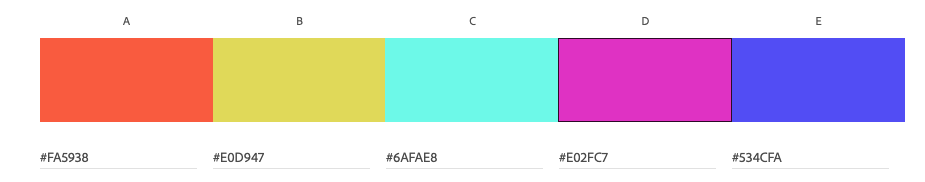
\includegraphics[width=1.0\textwidth]{images/paleta_de_cores_acessiveis.png}
        \caption{A imagem exemplifica uma paleta de cores onde todas as cores são acessíveis. Para a construção dessa paleta de cores foi utilizado o site do \textit{Adobe Color} \cite{ADOBE}.}
        \label{fig1:style}
\end{figure}  

É de extrema importância verificar como ficaria essas cores pela visão de pessoas que possuem algum tipo de daltonismo. Ao perceber que a paleta de cores ainda está com um contraste aceitável e de no mínimo 7:1 ela está pronta para o uso, seguindo a diretriz nível AAA de contraste \ref{Diretrizes nível AAA}. Na figura \ref{fig2:style} é possível observar os diferentes tipos de daltonismo e como a paleta de cores se comporta diante das limitações de visão de pessoas com daltonismo. Essa paleta foi criada utilizando as ferramentas de acessibilidade do \textit{Adobe Color Wheel} \cite{ADOBE}.
 \begin{figure}[ht]
        \centering
    	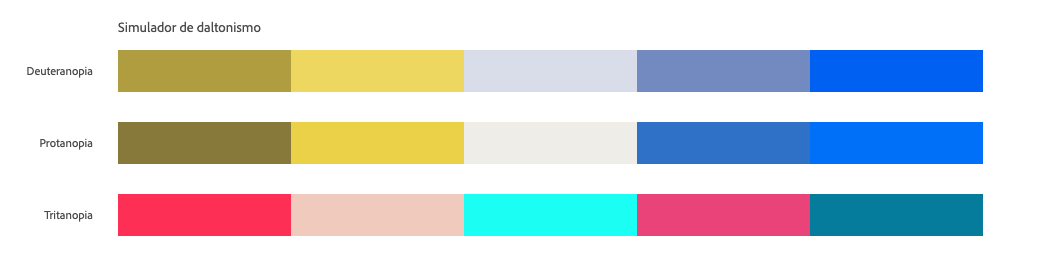
\includegraphics[width=1.0\textwidth]{images/paleta_daltonismo.png}
        \caption{A imagem simula o comportamento de uma paleta de cores acessível diante dos tipos de daltonismo.}
        \label{fig2:style}
\end{figure}  


\newpage

{\centerline{\textbf{Tipografia}}}
A tipografia não é apenas escolher uma fonte legal para o seu projeto, junto com ela devemos levar em consideração vários aspectos que são importantes e foram listados nas diretrizes: 
\begin{itemize}
    \item Espaçamento
    \begin{itemize}
        \item O espaçamento deve ser bem planejado para que seja possível aplicar um zoom de 200\%\ e ou ainda em caso de redimensionamento de tela o texto deve permanecer legível. \ref{Diretrizes nível AA}
    \end{itemize}
    \item Altura de linhas
    \begin{itemize}
        \item Sempre que houver um redimensionamento os textos não devem perder legibilidade. \ref{Diretrizes nível AA}
    \end{itemize}
    \item Hierarquia tipográfica
    \begin{itemize}
        \item Sempre que o conteúdo da tela for dividido em sessões, todas devem possuir títulos claros, com níveis de hierarquia bem definidos, para assim manter a hierarquia da informação de uma forma concisa. \ref{Diretrizes nível AAA}
    \end{itemize}
    \item Pesos, cores e contraste. 
    \begin{itemize}
        \item O contraste entre textos e telas também deve ser mantido num padrão de no mínimo 4:5:1. \ref{Diretrizes nível A}
    \end{itemize}
\end{itemize}

A figura \ref{fig3:tipografia} foi criada usando os recursos de acessibilidade presentes na ferramenta \textit{Adobe Color Wheel} \cite{ADOBE}. A partir da cor do texto e da cor de fundo é possível saber a proporção de contraste e se está dentro do esperado nas diretrizes WCAG \cite{WCAG20}.

\begin{figure}[ht]
    \centering
	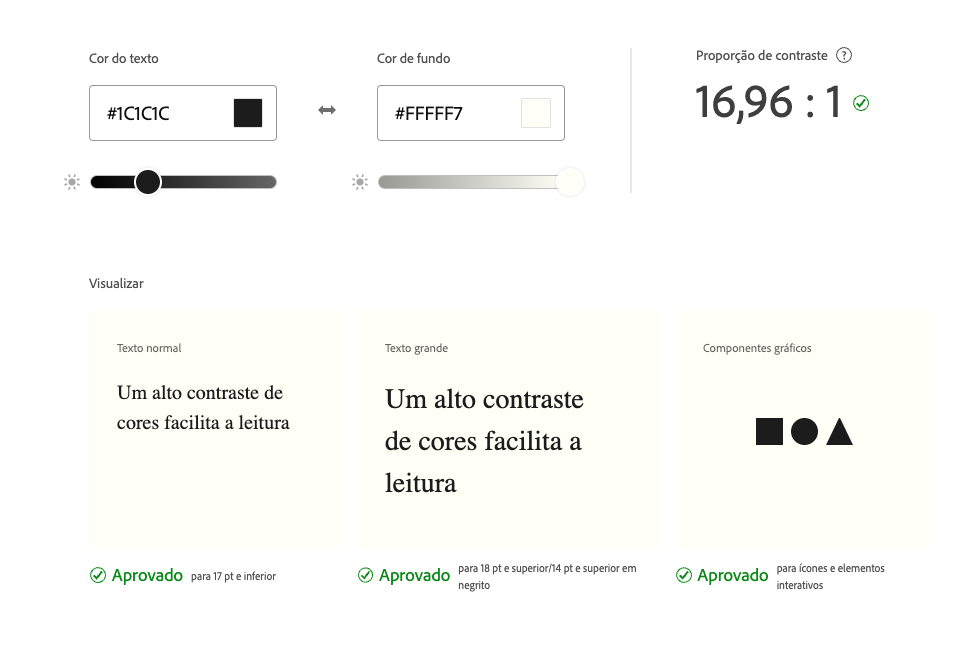
\includegraphics[width=1.0\textwidth]{images/contrast_check.png}
    \caption{A figura exemplifica a checagem de contraste entre texto e fundo realizado por meio do site  \textit{Adobe Color Wheel} \cite{ADOBE}}
    \label{fig3:tipografia}
\end{figure} 

\newpage
{\centerline{\textbf{Elementos da \textit{interface} do usuário}}}
Este tópico compreende os elementos que estarão presentes na \textit{interface}, logo serão apresentados exemplos e listagem desses componentes. Na construção desses elementos é feito o detalhamento visual, ou seja, os tamanhos, espaços, margens, cores que ele deve possuir como também os seus estados comportamentais, se houver um erro como ele se comporta, em caso de elemento focado como deve ficar o elemento.

Com o componente \textit{Card} da figura \ref{fig:UI_componentes} abaixo podemos analisar onde as diretrizes foram aplicadas e como elas impactam na construção de componentes mais complexos da \textit{interface} do usuário.  

\begin{figure}[ht]
        \centering
    	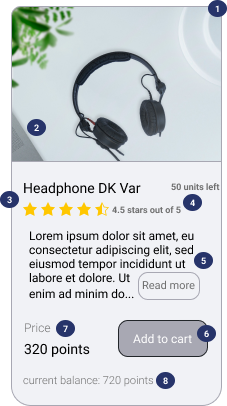
\includegraphics[width=0.38\textwidth]{images/ui-exemplo.png}
        \caption{Exemplo de um componente montado com elementos da interface do usuário}
        \label{fig:UI_componentes}
\end{figure}

Abaixo na tabela \ref{elementos de UI} foi referenciado os identificadores de 1 a 8 apontados na Figura \ref{fig:UI_componentes} com as diretrizes aplicadas em cada ponto juntamente com sua breve descrição. Foi especificado o nível em que cada diretriz se encontra. Para maiores detalhes sobre as diretrizes consultar o apêndice \ref{sec:apendice}.
{


\noindent\begin{minipage}{\linewidth}
\centering
\captionof{table}{Elementos de UI}\resizebox{\linewidth}{!}{%
\begin{tabular}{|c|l|l|c|p{400px}|} 
\hline
\rowcolor[HTML]{ECF4FF} 
{\color[HTML]{333333} Identificador & Diretriz} & Nome & Nível & Descrição \\ 
\hline
    1 & 3.2.1  &
       Em foco & A & O foco sempre deve se manter durante a navegação, guiando o usuário e evitando mudanças que causem desorientação. \\ 
       \cline{2-5} & 2.4.7 & Foco visível & A & Ao se interagir por teclado, qualquer pessoa deve conseguir identificar qual é a sua localização na tela através de um foco visível. \\ 
        \cline{2-5} & 1.3.1 & Informações e Relações & A & As estruturas da tela devem ser construída de forma que sua arquitetura de informação faça sentido tanto para todos, sejam ouvintes ou leitores. \\ 
        \cline{2-5} & 1.3.2 & Sequência com significado & A & A apresentação das informações na tela sempre deverá ter uma sequência lógica. \\ 
       \hline
    2 & 1.1.1 & 
        Conteúdo Não Textual & A & Todo o conteúdo não textual que é exibido ao usuário tem uma alternativa textual que serve a um propósito equivalente.\\
        \cline{2-5} & 1.4.11 & Contraste Não textual & AA & apresentação visual a seguir tem um relação de contraste de pelo menos 3:1 contra cor(es) adjacente(s).\\
        \hline
    3 & 1.4.3 & 
        Contraste (mínimo) & AA & Textos devem ter uma relação de contraste entre primeiro e segundo plano de ao menos 4.5:1.\\
        \cline{2-5} & 2.4.6 & Cabeçalhos e rótulos  & AA & Todos os títulos e rótulo devem descrever claramente a finalidade dos conteúdos, não deve haver ambiguidade em seu entendimento.\\
    \hline
    4 & 1.4.6 & 
        Contraste (melhorado) & AAA & Textos devem ter uma relação de contraste entre primeiro e segundo plano de ao menos 7:1.\\
        \cline{2-5} & 1.4.11 & Contraste Não textual & AA & A apresentação visual a seguir tem um relação de contraste de pelo menos 3:1 contra cor(es) adjacente(s).\\
    \hline 
     5 & 2.4.7 & 
        Foco visível  & A & Ao se interagir por teclado, qualquer pessoa deve conseguir identificar qual é a sua localização espacial na tela através de um foco visíve\\
        \cline{2-5} & 3.2.1 & Em foco & A & O foco sempre deve se manter durante a navegação, guiando o usuário e evitando mudanças que causem desorientação.\\
        \cline{2-5} & 2.5.5 & Tamanho da área clicável & AAA & O tamanho das áreas acionáveis por clique ou toque devem possuir no mínimo 44x44 pixeis de espaçamento\\
        \cline{2-5} & 2.5.3 & Rótulo no Nome acessível & A & Rótulos em botões, ícones acionáveis ou qualquer controle interativo, devem ter uma descrição significativa.\\
        \cline{2-5} & 1.4.12 & Espaçamento de texto & AA & Sempre que houver um redimensionamento os textos não devem perder legibilidade\\
        \cline{2-5} & 1.4.13 & Conteúdo em foco por mouse ou teclado & AA & Conteúdos adicionais não devem ser acionados apenas com foco por mouse ou teclado.\\
        \cline{2-5} & 2.1.1 & Teclado & A & Todas as funcionalidades devem ser acionadas via teclado. \\
        \cline{2-5} & 2.1.2 & Sem bloqueio de teclado & A & Ao se interagir via teclado, a navegação por todos os elementos ”clicáveis”deve ocorrer sem que haja bloqueios ou interrupções.\\
        \cline{2-5} & 2.1.3 & Teclado (sem exceção) & AAA & Todas as funcionalidades devem ser acionadas via teclado, sem exceção.\\
    \hline 
    6 & 2.4.3 & 
        Ordem do foco & A & A interação por elementos focáveis na tela sempre deverá ser sequencial e lógica de acordo com o conteúdo apresentado.\\
        \cline{2-5} & 2.4.7 & Foco visível & A & Ao se interagir por teclado, qualquer pessoa deve conseguir identificar qual é a sua localização na tela através de um foco visível. \\
        \cline{2-5} & 3.2.3 & Navegação consistente & AA & Deve-se manter a consistência com relação ao formato de apresentação, interação e localização na tela. \\
        \cline{2-5} & 1.4.12 & Espaçamento de texto & AA & Sempre que houver um redimensionamento os textos não devem perder legibilidade\\
        \cline{2-5} & 1.4.13 & Conteúdo em foco por mouse ou teclado & AA & Conteúdos adicionais não devem ser acionados apenas com foco por mouse ou teclado.\\
        \cline{2-5} & 2.1.1 & Teclado & A & Todas as funcionalidades devem ser acionadas via teclado. \\
        \cline{2-5} & 2.1.2 & Sem bloqueio de teclado & A & Ao se interagir via teclado, a navegação por todos os elementos ”clicáveis”deve ocorrer sem que haja bloqueios ou interrupções.\\
        \cline{2-5} & 2.1.3 & Teclado (sem exceção) & AAA & Todas as funcionalidades devem ser acionadas via teclado, sem exceção.\\
        \cline{2-5} & 2.4.8 & Localização & AAA & Qualquer pessoa deve conseguir se localizar ou se orientar facilmente em qualquer nas telas.\\
        \cline{2-5} & 3.2.4 & Identificação consistente & AA & Deve-se manter a consistência com relação a diferentes formatos de elementos, mas que possuem uma mesma funcionalidade.\\
        \cline{2-5} & 2.5.2 & Cancelamento de acionamento & A & Deve se fornecer um modo de cancelar acionamentos feitos de forma não proposital.\\
    \hline
    7 & 1.4.3 & 
        Contraste (mínimo) & AA & Textos devem ter uma relação de contraste entre primeiro e segundo plano de ao menos 4.5:1.\\
        \cline{2-5} & 1.4.6 & Contraste (melhorado) & AAA & Textos devem ter uma relação de contraste entre primeiro e segundo plano de ao menos 7:1.\\
    \hline
    8 & 4.1.3 & 
        Mensagens de status & AA & Qualquer tipo de mensagem que é resultado de uma ação deve ser transmitida sem que ocorra uma mudança de foco na tela.\\
    \hline

\end{tabular}
}
\label{elementos de UI}

\end{minipage}

}}


\subsection{Fase 2: Adaptação e construção da \textit{interface} do usuário acessível e usável usando o guia de acessibilidade e \textit{style guide}}
{A segunda fase se concentrou na adaptação da \textit{interface} do usuário e na construção de novos componentes para o \textit{e-commerce}, sempre seguindo os guias. Nessa fase o foco principal se dividiu em duas vertentes:
\begin{itemize}
\item Criar abordagens inteligentes para problemas de acessibilidade em imagens, formulários e navegação e a adaptação de componentes com \textit{HTML} \cite{HTML} não semântico para semântico.
\item  Adaptar e criar componentes para que as tecnologias assistivas pudessem entendê-los corretamente e assim ter uma a navegação por teclado eficaz.

\end{itemize}
}
\subsubsection{Abordagens inteligentes e adaptação de componentes}
{\begin{itemize}
    \item O primeiro passo a se fazer foi organizar o \textit{HTML} \cite{HTML} de forma logica e semântica, onde cada \textit{tag} deve ser usada para o fim que ela foi criada seguindo uma ordem que seja compreensível além de corresponder ao conteúdo desejado. Nesse ponto em um sistema legado muitos componentes estavam escritos de maneira errada, algumas \textit{tags} \textit{HTML} \cite{HTML} estavam sendo usadas com um proposito diferente do que ela foi criada e para esses casos utilizamos a abordagem \textit{WAI-ARIA} \cite{WAI-ARIA} para que o leitor conseguisse entender o que era cada \textit{tag} daquela e também fosse possível fazer a navegação via teclado.

\vspace{1.5cm}
{\centerline{\textbf{Caso de uso 1}: Transformando botão inacessível em acessível} 
Adaptação de um botão que foi construído de forma não acessível e por isso não era lido por leitores de tela e nem navegável via teclado. Nesse exemplo, foi usado o atributo \lstinline{role} do \textit{WAI-ARIA}\cite{WAI-ARIA} para dar o comportamento de botão a essa \lstinline{div} e com isso ganhar todos os atributos e comportamentos que um botão teria.

\begin{lstlisting}[language=html, caption=Componente de botão antes de receber boas praticas e acessibilidade]
    <div
        className="button__add"
        onClick={event => onClick(event)}
    >
      Adicionar ao carrinho 
    </div>
\end{lstlisting}}
{\begin{lstlisting}[language=html,caption=Adaptação do componente de botão usando \textit{WAI-ARIA} \cite{WAI-ARIA}]
<div 
    role="button" 
    tabIndex="0" 
    className="button__add"
    onClick={event => onClick(event)}
    onKeyDown={event => keyHandler(event, props.onClick)}
    {...props}
>
    Adicionar ao carrinho
</div>
 
\end{lstlisting}}

\vspace{1.5cm}
{\centerline{\textbf{Caso de uso 2}: Adaptação e construção de imagens acessíveis.} 
As imagens que possuem algum tipo de conteúdo devem ser acessíveis, elas precisam de alguma descrição, seja ela visível ou não. Existe o atributo \lstinline{alt} para a \textit{tag} \lstinline{img}, onde ele serve para descrever o que está presente na imagem. Essa descrição do \lstinline{alt} não aparece visualmente, mas ela é lida pelo leitor de tela, quando o usuário, navegando pelo teclado, passar pela imagem.}
{\begin{lstlisting}[language=html,caption=usando atributo \lstinline{alt}]
<img src="headphone.jpg" alt="Headphone na cor preto"> 
\end{lstlisting}}
\item Caso haja necessidade de fornecer uma informação contextualizada é necessário fazer uso do atributo \lstinline{title}. Nesse caso, a maioria dos leitores de tela lerá o texto alternativo, o atributo de título e o nome do arquivo. Além disso, os navegadores exibem o texto do título como dicas de ferramentas quando estão sobre o \textit{mouse}. Com a chegada do \textit{HTML 5} \cite{HTML} surgiram dois novos elementos o \lstinline{<figure>} e \lstinline{figcaption>}, que devem associar uma figura a uma legenda. 
{\begin{lstlisting}[language=html,caption=usando atributo alt]
<figure>
  <img src="headphone.jpg" alt="Headphone na cor preto"> 
  <figcaption>Headphone com microfone acoplado na cor preta, com um fio de ótima construção</figcaption>
</figure>
\end{lstlisting}}

\item  Ainda temos os casos onde as imagens são apenas decorativas e como elas não carregam conteúdo elas devem ser ignoradas pelos recursos de tecnologia assistivas. Para esse caso nós temos três tipos de abordagens: 
\begin{itemize}
\item Por ser decorativa a melhor abordagem é incluí-las na página como imagens de fundo através de \textit{CSS} \cite{CSS} E caso a imagem transmita significado ao conteúdo, mas tenha sido inserida via \textit{CSS} \cite{CSS}, pode-se utilizar recursos \textit{WAI-ARIA}\cite{WAI-ARIA}.
{\begin{lstlisting}[language=html,caption=adicionando imagem via CSS]
<style>
div {
    background-image:url("./images/headphone-preto.png");
}
</style>
\end{lstlisting}}
\item Em casos de imagens que usam a \textit{tag} \lstinline{img} basta ter uma descrição \lstinline{alt} vazia. Isso faz com que os leitores de tela reconheçam a imagem mas não tentem descreve-la. A razão para usar um \lstinline{alt} vazio ao invés de não incluí-lo é porque muitos leitores de tela anunciam o URL da imagem inteira se nenhum \lstinline{alt} for fornecido.
{\begin{lstlisting}[language=html,caption=usando atributo \lstinline{alt} vazio]
<img src="logotipo.jpg" alt=""> 
\end{lstlisting}}

\item Em casos de imagens incluídas em tags que não são \lstinline{img} podemos fazer uso o atributo \textit{ARIA role} \cite{WAI-ARIA} \lstinline{(role="presentation")}, isso também impede que os leitores de telas leiam textos alternativos.
{\begin{lstlisting}[language=html,caption=usando atributo role="presentation"]
<div role="presentation" src="logotipo.jpg" alt="" />
\end{lstlisting}}
\end{itemize}


 
\end{itemize}}

{

\vspace{1.5cm}
{\centerline{\textbf{Caso de uso 3:} Criando formulários acessíveis.} }


\begin{itemize}
    \item O primeiro passo para criar um formulário acessível é criar uma estrutura \textit{HTML} \cite{HTML} com sequência lógica, essa sequencia é definida pela ordem que se encontra o \textit{HTML} \cite{HTML}. Fazendo isso a navegação pelos campos do formulário ficará mais fácil tanto por teclado quanto para leitores de tela. 
    \item A associação de um campo de entrada a um rótulo fará diferença para o usuário final. E quando não for possível fazer essa associação por tags \textit{HTML} \cite{HTML} existe outras opções como a forma \textit{WAI-ARIA} \cite{WAI-ARIA} usando o atributo \lstinline{aria-label}.
    \item É necessário o fornecimento de instruções claras sobre os dados de entradas pedidos no campo. As entradas devem ser facilitadas, retire caracteres especiais em campos numéricos e etc. 
    \begin{itemize}
        \item Para campos com obrigatoriedade de dados, deve-se ter um indicador visual e escrito de obrigatoriedade. O atributo \lstinline{required} auxilia no quesito de obrigatoriedade de um campo.
        \item Podemos adicionar também o atributo de estado \lstinline{aria-invalid} que pode ter os valores \textit{true} ou \textit{false} para indicar se o campo está válido ou inválido.
    \end{itemize}
    \item A identificação e descrição de erros de entrada e confirmação de envio de informações devem ser claras para o usuário. 
    \begin{itemize}
        \item A indicação do erro é feita de três formas: com uma cor, um texto informativo e um ícone de alerta. Assim, não usamos somente uma forma para representar esta informação, beneficiando pessoas sem deficiência visual, com deficiências cognitivas, que usam leitor de telas ou que possuem daltonismo;
        \item Uma área para mensagem informativa em um formulário sempre será bem-vinda. Esta área de mensagem informativa do formulário possui os atributos \lstinline{role="alert"}, que avisa que é uma mensagem de alerta e \lstinline{aria-live="assertive"} que informa que é um campo que pode sofrer modificações no conteúdo e o leitor de telas é informado quando há modificação neste campo;
    \end{itemize}
    \item É necessário haver distinção visual de qual campo está recebendo o foco no momento, mesmo aplicando o \lstinline{outline} padrão do navegador. A customização desse \lstinline{outline} pode ser feita para que ele sempre fique visível qual campo contém o foco.
    
    {\begin{lstlisting}[language=html, caption=Formulário acessível]
    <form>
        <output id="formMessage" role="alert" aria-live="assertive" tabindex="0" class="error">
            O formulário apresenta erros que impedem a finalização do seu cadastro. Confira se todos os campos obrigatórios foram preenchidos e tente novamente.
        </output>

        <p>
            <label for="email1">
                E-mail <span class="required">(obrigatório)</span>:
            </label>
            <input type="email1" name="email1" id="email1" required="" aria-invalid="true" aria-describedby="emailMessage">
            <span class="fieldMessage" id="emailMessage">
                O e-mail não pode ficar em branco e deve ser válido.
            </span>
          </p>
  
          <p>
            <label for="phone1">
                Telefone <span class="optional">(opcional)</span>:
            </label>
            <input type="tel" name="phone1" id="phone1" aria-describedby="phoneTip">
            <span class="fieldTip" id="phoneTip">
                Formato: (99) 99999-9999.
            </span>
          </p>

        <button class="formButton" id="formButtonARIA" type="submit">Finalizar cadastro</button>
    </form>
    \end{lstlisting}}
    
    \begin{figure}[ht]
  		\center
        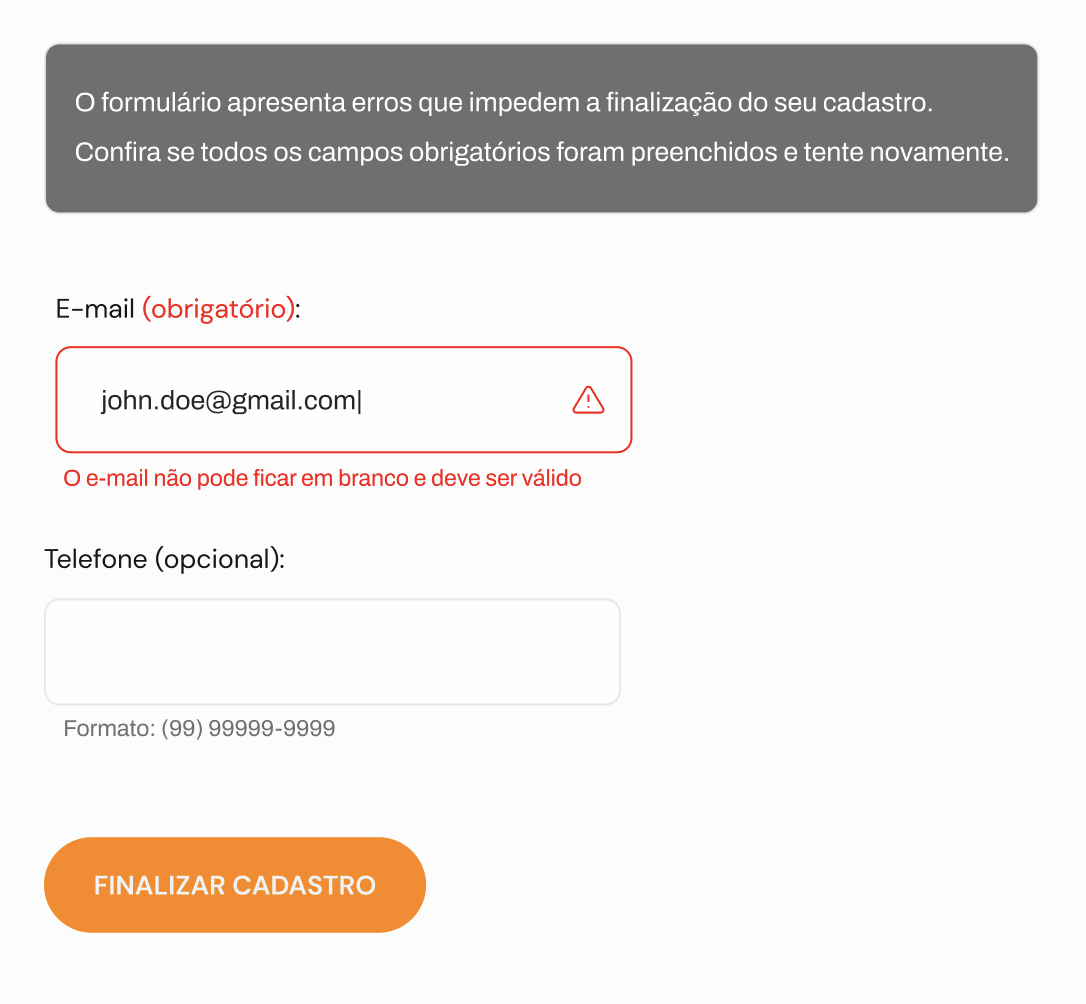
\includegraphics[width=0.7\textwidth]{images/form-acessivel.png}
        \caption{Formulário criado usando as técnicas listadas acima}
    \end{figure} 
\end{itemize}
}
\subsubsection{Adaptação de componentes para o uso de leitores de telas e navegação por teclado}
{Antes de falar de adaptação de componentes é necessário entender como funciona o leitor de telas. O leitor de telas basicamente é um software que vai percorrendo textos e imagens e lendo em voz alta tudo o que ele encontra na tela, a partir do momento que o usuário começa a interagir com o software para efetuar uma navegação ele vai percorrendo o documento saltando entre elementos interativos e cabeçalhos. Para que essa navegação ocorra tudo deve está funcionando direito, pois caso contrário o usuário pode se perder na página e ter dificuldades em entender como a informação está organizada. No leitor de telas a navegação ocorre de três maneiras: 
\begin{itemize}
    \item Navegação com as setas direcionais: Usando a navegação por setas direcionais o usuário consegue acessar as informações textuais.
    \item Navegação por tecla \textit{tab}: O leitor sai pulando para os links espalhados na página.
    \item Navegação com a tecla h: O leitor salta entre os cabeçalhos marcados na página.
\end{itemize}



{
\vspace{1.5cm}
{\centerline{\textbf{Caso de uso 1:} Navegação por cabeçalho.}}.

Cabeçalhos compõem a hierarquia de informação do site, essa hierarquia é usada pelos leitores de tela para navegação dentro da página. A grande maioria dos leitores de tela dispõem de atalhos para acesso rápido aos cabeçalhos marcados na página. Para garantir que tecnologias assistivas acessem o conteúdo dos cabeçalho sem sua ordem de importância é preciso tomar alguns cuidados: 
\begin{itemize}
    \item Cuidado com múltiplas \textit{tags} \lstinline{h1} na página. Mesmo que haja separação de contexto para a utilização de mais de um \lstinline{h1} por página o leitor de tela não consegue identificar a diferença e a importância de \lstinline{h1} contidos em outras \textit{tags}.
    \item Para essa navegação funcionar, o código precisa ter sido escrito com a semântica correta, ou seja, cabeçalhos devem ser definidos como cabeçalhos e não usar qualquer outro artificio visual para se assemelhar a um cabeçalho. 
\end{itemize}
{\begin{lstlisting}[language=html,caption=cabeçalhos com hierarquia]
<h1>Cabeçalho Principal</h1>
<p>Exemplo de um texto de um parágrafo</p>
<h2>Cabeçalho Secundário</h2>
<p>Mais texto de um parágrafo.</p>
\end{lstlisting}}

\vspace{1.5cm}
{\centerline{\textbf{Caso de uso 2:}  Navegação por tabulação e leitores de tela}}
{
{
A ordem da navegação por tabulação é derivada da forma como o \textit{layout} do \textit{site} está escrito, contudo a ordem padrão pode não corresponder necessariamente a ordem visual. Ao utilizar a tecla \textit{tab}, o leitor de tela realiza o foco e lê em voz alta os \textit{links} e componentes interativos presentes na página.  A tabulação é utilizada somente para navegar entre os \textit{links}, e com isso todos os \textit{links} terão que ser localizados através destas duas formas, com a tabulação ou com as setas. O que diferencia uma forma da outra, é que com as setas, o usuário poderá ler toda a página (incluindo texto entre os \textit{links}), e com a tabulação, o usuário só pode localizar os \textit{links}, botões, campos de edição, e caixas de seleção.


Navegar por entre os \textit{links} é uma forma de observar o texto rapidamente, especialmente se os usuários estiverem tentando encontrar uma seção específica do \textit{website}. Para ter uma navegação por tabulação eficiente é preciso passar por alguns pontos: 
\begin{enumerate}
    \item Ordene de forma lógica e intuitiva a leitura e tabulação. Preparar o \textit{HTML}\cite{HTML} para ter uma navegação consistente e eficaz é essencial para o bom funcionamento da navegação atrelada a leitores de tela. 
    \item Usar a tecla \textit{tab} para passar pelos links e controles de formulários
    das páginas, certificando-se de que todos os links e controles de formulários podem ser acessados, bem como se os links indicam claramente para onde levam. 
    \begin{itemize}
        \item Com atributo \lstinline{tabindex} é possível definir uma ordem de foco nos elementos dispostos na tela. Usando o \lstinline{tabindex=0} é inserido um elemento na ordem natural de tabulação e com \lstinline{tabindex="-1"} um elemento é removido da ordem e tabulação.

{\begin{lstlisting}[language=html,caption=Uso do atributo tabindex]
<label>
    Primeiro na lista de tabulação:<input type="text">
</label>
<div tabindex="0">
Próximo item na lista de tabulação, mesmo não sendo um elemento que receberia o foco natural
</div>
<div>Não será focado pois está sem o tabindex</div>
\end{lstlisting}}
        \item Adicione o atributo \lstinline{title} aos \textit{links}, ele mostrará uma descrição do lugar pra onde o \textit{link} leva, melhorando a navegação.
{\begin{lstlisting}[language=html,caption=usando o atributo title]
<a href="#" onclick="abrePopup()" onkeypress="abrePopup()" title="Abre uma janela pop-up com Javascript">Ver mais informações</a>
\end{lstlisting}}
    \end{itemize}
    \item Forneça âncoras para ir direto a um bloco de conteúdo. São comumente chamados de \textit{landmarks} é um tipo de região em uma página \textit{web} a qual uma pessoa pode querer acessá-la rapidamente. Um dos principais benefícios em se usar pontos de referência é a possibilidade de o usuário acessar diretamente uma região da página sem a necessidade de seguir a ordem natural do conteúdo. Isso é especialmente relevante para o caso de pessoas que utilizam leitores de tela para navegar na \textit{web}. Para essa abordagem é muito utilizado o CSS \cite{CSS} deixando-os \textit{links} invisíveis e apenas disponíveis quando a navegação por tabulação se iniciar. 
{\begin{lstlisting}[language=html,caption=usando landmarks]
<div role="heading" id="cabecalho"> 
  <h1>O Cabeçalho</h1> 
  <a href="#conteudo" accesskey="p">Pular para o conteúdo principals</a> 
</div> 
<div role="navigation" id="navegacao"> conteúdo da navegação </div>
<div role="main" id="conteudo"> conteúdo da main </mdiv>
\end{lstlisting}}
    \item É aconselhável não tabelas para diagramação. As tabelas devem ser utilizadas apenas para dados tabulares e não para efeitos de disposição dos elementos na página. O leitor de telas sairá pulando por cada campo das tabelas e o usuário poderá ficar perdido na navegação. Para efeitos de diagramação a melhor opção está na utilização do \textit{CSS} \cite{CSS}.
    \item Utilização de separação dos \textit{links} adjacentes. Em uma sequência de \textit{links}, além do espaço, é importante o uso de separadores ou elementos do HTML \cite{HTML} adequados para que as pessoas com deficiência identifiquem claramente onde termina e começa um novo \textit{link}. É recomendado o uso de listas , em que cada elemento dentro da lista é um link.
{\begin{lstlisting}[language=html,caption=separando \textit{links} adjacentes]
<ul id="menu">
    <li> <a href="home.html">Home</a></li>
    <li> <a href="pesquisa.html">Pesquisa</a></li>
</ul>
\end{lstlisting}}
    \item É desencorajado a abertura novas instâncias sem a solicitação do usuário. O impedimento de  redirecionamento automático de páginas é algo necessário. Forçar a abertura de \textit{links} em uma nova janela não é algo esperado e o usuário se perderá na navegação. Caso haja implementação dessa funcionalidade, a utilização de \textit{link} é atrelada a ter uma iconografia óbvia e explicativa, usando pseudo-elemento \lstinline{::after} no CSS \cite{CSS}. No CSS \cite{CSS} o conteúdo de pseudo-elementos é lido em voz alta por leitores de tela, portanto é de extrema importância de que o conteúdo seja com informações relevantes.
    \item O conteúdo deve possuir o foco por mouse ou teclado e esse foco deve ser visível. Para pessoas com baixa visão, é muito importante que seja possível perceber facilmente onde está o foco do teclado, garantindo uma maior facilidade de navegação. A pseudo-classe \lstinline{:focus} é utilizada para definir o estilo de qualquer elemento HTML \cite{HTML} que receber o foco do teclado, como \textit{links} e elementos de formulário.
{\begin{lstlisting}[language=html,caption=usando o foco visível]
a:focus, a:hover {
    border: 2px solid #F00;
}
\end{lstlisting}}
    \item Todas as funcionalidades que estão disponíveis via mouse deverão estar disponíveis para serem acionadas via teclado. Só dessa forma o site estará totalmente acessível para pessoas com deficiências visuais. 
\end{enumerate}
}
}
}


\subsection{Fase 3: Construção do dashboard acessível}
{Para a construção do \textit{dashboad} com gráficos foi utilizado a biblioteca D3.js \cite{D3} que é usada para visualização de informação. Essa biblioteca permite que seja construído aplicações em que os dados entram puros e são dinamicamente associados em representações gráficas. Com o D3 o DOM \cite{DOM} (Document Object Model)  pode ser facilmente manipulado já que ele usa usa os padrões da web como HTML \cite{HTML}, CSS \cite{CSS}, SVG para renderizar gráficos de visualização poderosos.

\begin{figure}[ht]
  	\center
    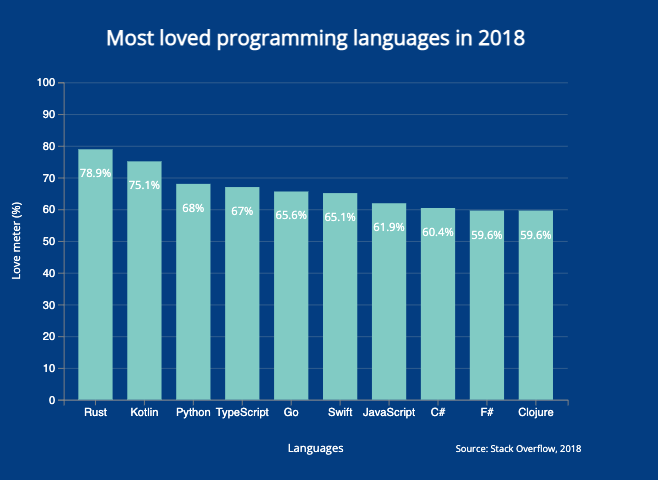
\includegraphics[width=0.7\textwidth]{images/exemplo-graf-d3.png}
    \caption{Exemplo de um gráfico desenvolvido com D3.js}
\end{figure} 

}

\vspace{1cm}
{\centerline{\textbf{Construção de gráficos com D3.js}}}
No \textit{e-commerce} foi decidido não construir o gráfico inteiramente com D3.js \cite{D3}, pois a abordagem normal presente não facilitaria o reaproveitamento para a criação dos componentes. Quando um gráfico é plotado somente com D3.js \cite{D3} pode haver problemas de performance, visto que o React \cite{REACT} não estava preparado para esse tipo de renderização contínua criada ao se aplicar filtros e interações nos gráficos. Dessa forma, a abordagem mais coerente era usar as \textit{tags} HTML \cite{HTML} normais e quando era necessário feito a criação do elementos e interações usando o D3.js \cite{D3}.

Para a manipulação do DOM (Document Object Model) \cite{DOM}, é necessário aprender a utilizar os recursos presente no D3 \cite{D3}. A biblioteca usa JavaScript para realizar a maioria das tarefas de seleção, transição e vinculação de dados.

A primeira coisa necessária para construir um gráfico com D3.js \cite{D3} é adicionar a biblioteca ao projeto, seja por gerenciador de pacotes ou por importação direta na \textit{tag} \lstinline{script}. Feito isso, é preciso ter uma \textit{tag} como base onde as partes do gráfico serão injetadas, geralmente é usada a \textit{tag} \lstinline{svg} pois ela auxilia na construção de formas geométricas que será utilizado no gráfico. Após adicionar a \textit{tag} \lstinline{svg} precisamos adicionar uma nova \textit{tag} \lstinline{g} para que o gráfico comece a tomar forma, essa \textit{tag} \lstinline{g} é um recipiente utilizado para agrupar objetos.

Para começar a desenhar qualquer tipo de gráfico é necessário colocar os eixos das abscissas e ordenadas. Na construção desses eixos é deve-se estabelecer qual o domínio de cada  eixoe após isso iniciar a construção das escalas, para que assim todos os dados consigam ser comportados dentro dos limites estabelecidos pela escala. O próprio D3 \cite{D3} já fornece alguns tipos de funções que nos auxiliam na criação dessas escalas, as funções são: \lstinline{d3.scaleBand()}, esta função divide o intervalo em n bandas onde n é o número de valores na matriz de domínio e \lstinline{d3.scaleLinear}, que é usada para criar um ponto de escala visual. Será criado duas escalas, uma para o eixo X usando a \lstinline{d3.scaleBand()} e outra para o eixo Y usando a \lstinline{d3.scaleLinear}.

O próximo passo é criar por fim o conteúdo do gráfico de forma visual. Com o apoio de dados vindos de uma API podemos atribuir ao longo do eixo X e do eixo Y os valores e formas visuais necessárias. Utilizando a função \lstinline{attr} será possível definir os atributos do elemento, uma vez que essa função recebe dois parâmetros o nome do atributo e o valor desse atributo. Graças a essa função podemos definir altura, largura e os valores de cada ponto dos eixos.

Depois que todos os valores dos gráficos estiverem corretamente plotados podemos lidar com as interações que estarão no gráfico. Todas as interações presentes via mouse devem também estarem disponíveis via teclado, ou seja, se houver um interação de clique de mouse deve haver uma interação de pressão de tecla. Para auxiliar na construção dessas interações pode-se usar a função \lstinline{.on()} que ficará responsável por agir como um \textit{event listener} de um elemento, onde qualquer tipo de interação será percebida. Essa função recebe dois argumentos, sendo o primeiro o tipo de evento e o segundo uma função que será disparava quando essa evento for detectado. 


\vspace{1cm}
{\centerline{\textbf{Tornando os gráficos acessíveis a leitores de tela}}}
{Além de tornar os gráficos acessíveis a qualquer tipo de navegação e interação é preciso que as imagens e os elementos presentes também estejam acessíveis e para isso existem algumas abordagens eficientes.  

O gráfico exemplificado abaixo \ref{fig:grafico-d3} foi construído levando em consideração as barreiras de acessibilidade que um deficiente visual frequentemente se depara. Logo, para diminuir essas barreiras as decisões tiveram como apoio as diretrizes WCAG \ref{sec:apendice} que se adéquam ao proposito do \textit{e-commerce} e a construção do gráfico com D3.js \cite{D3} se deu com o apoio das mesmas. 


\begin{figure}[ht]
  	\center
    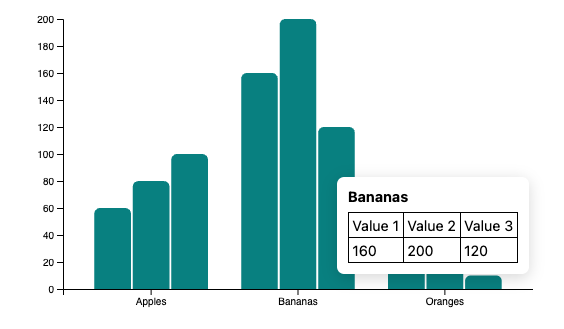
\includegraphics[width=0.7\textwidth]{images/barchart-tooltip.png}
    \caption{Gráfico do tipo de barras estacadas com \textit{tooltip} de visualização.}
    \label{fig:grafico-d3}
\end{figure} 

}


{

{Tomando como exemplo a figura \ref{fig:grafico-d3}, a tabela \ref{Barreiras e decisões na construção de um gráfico acessível} logo abaixo exemplifica cada barreira de acessibilidade e sua respectiva tomada de decisão.}
\vspace*{20px}

\noindent\begin{minipage}{\linewidth}
\centering
\resizebox{\linewidth}{!}{%
\begin{tabular}{|l|l|p{400px}|} 
\hline
\rowcolor[HTML]{ECF4FF} 
{\color[HTML]{333333}  Barreira de acessibilidade} &
  Tomada de decisão  \\ 
\hline
\begin{tabular}[c]{@{}l@{}}Falta de atributo \lstinline{alt} ou atributo não \\ descritivo\end{tabular} &
  \begin{tabular}[c]{@{}l@{}}Se faz necessário o uso do atributo \lstinline{alt}. Os leitores de tela falam texto alternativo sem permitir que os usuários acelerem \\ou pulem,  portanto, as informações sejam descritivas, mas sucintas.\end{tabular} \\ \hline
Existência de títulos não objetivos &
  \begin{tabular}[c]{@{}l@{}}Adicionar um título claro em cada gráfico plotado: A primeira coisa que será lida em um gráfico é o título,   isso \\facilitará a experiência dos usuário de leitor  de tela, que ao  perceber que aquele gráfico não é o que  ele precisa \\ ver no momento poderá pular a leitura ou modificar o filtro em questão.\end{tabular} \\ \hline
Falta de rotulação nos dados &
  \begin{tabular}[c]{@{}l@{}}Legendas podem ser não eficientes para usuários daltônicos ou deficientes visuais que podem ter dificuldade em \\ combinar as cores do gráfico  com as da legenda.  Rotulando também diminuirá o trabalho de varredura para frente \\ e para trás tentando combinar a legenda com os dados. \end{tabular}\\ \hline
Dados fornecidos apenas por gráficos &
  \begin{tabular}[c]{@{}l@{}}Forneça os dados de algum outro modo que não somente por gráficos: Incluir um link para um CSV ou outro formato \\ de dados legível por máquina  para que pessoas com deficiência visual possam navegar pelos dados do gráfico com\\ um leitor de tela é essencial.\end{tabular} \\ \hline
  
\begin{tabular}[c]{@{}l@{}}Pouco contraste entre o fundo do \\ gráfico e o conteúdo do gráfico\end{tabular} &
  \begin{tabular}[c]{@{}l@{}}Verifique se o contraste de cores do gráfico está dentro dos padrões da WCAG \cite{WCAG}.\end{tabular} \\ \hline
  
\begin{tabular}[c]{@{}l@{}}Separação não clara entre os \\setores dos gráficos\end{tabular} &
  \begin{tabular}[c]{@{}l@{}}Utilizar espaços em branco para separar gráficos que são empilhados.  O uso criterioso do espaço em branco aumenta\\ a legibilidade, ajudando a demarcar e distinguir as diferentes seções sem depender apenas da cor. Isso também pode \\ complementar as opções de cores acessíveis,  ajudando os usuários a distinguir a diferença entre as cores que identificam \\seções separadas.\end{tabular} \\ \hline

\end{tabular}%
}
\captionof{table}{Barreiras e decisões na construção de um gráfico acessível}
\label{Barreiras e decisões na construção de um gráfico acessível}

\end{minipage}

}

\vspace{1cm}
{\centerline{\textbf{Gráficos como componentes reutilizáveis}}}


{Quando se trabalha com React \cite{REACT} ao se criar um componente devemos garantir que esse ele possa ser reutilizável, para que isso seja possível no momento da criação de cada componente deve-se ter em mente que quanto menor e mais genérico for o componente mais ele será escalável e com isso facilitará a construção de componentes maiores.

Para facilitar a construção como módulos separados cada tipo de gráfico se tornou um componente reutilizável. Em cada componente desses contaria com suas funções e particularidades, porém com a flexibilidade de ser um componente genérico, onde todos os dados são populados através de propriedades que são repassadas do componente pai para o componente filho. 



}
}


\subsection{Fase 4: Testes e avaliações de acessibilidade}
{Durante e após a construção do e\textit{e-commerce} de acordo com os
padrões \textit{web} e as diretrizes de acessibilidade, é necessário efetuar testes para garantir sua acessibilidade. Todos os testes descritos nessa seção foram executados por pessoas que não são os \textit{stakeholders} do projeto, porém para cobrir o máximo de casos de testes possível esses testes foram abordados e executados de dois modos: 
\begin{itemize}
\item Avaliação automática: São as avaliações feitas de maneira automática por meio de \textit{plugins} de verificação e de \textit{websites} de validação.
\begin{itemize}
    \item \href{https://chrome.google.com/webstore/detail/accessibility-developer-t/fpkknkljclfencbdbgkenhalefipecmb?hl=pt-BR}{\textit{Google Accessibility Developer Tools}} ({Plugins} para navegador \textit{Chrome}).
    \item \href{https://developer.chrome.com/docs/devtools/}{\textit{DevTools}}({Plugins} para navegador \textit{Chrome}).
    \item \href{https://contrastchecker.com/}{Contrast Checker} (\textit{website} - Validação de contraste de cores).
\end{itemize}
\item Avaliações manuais: Essa etapa se deu usando o leitor de tela e a navegação por teclado, onde foi checado se todos os comportamentos e ações esperados estão sendo realmente respeitados e executados.
\end{itemize}
}

\subsection{Tecnologias utilizadas} 
{A linguagem de programação JavaScript foi escolhida para a elaboração deste trabalho devido a sua grande relevância no frontend. Entre as principais bibliotecas utilizadas neste projeto destaca-se:
\begin{itemize}
\item \textit{HTML \href{https://developer.mozilla.org/pt-BR/docs/Web/HTML}{HTML}: é uma linguagem de marcação utilizada na construção de páginas na \textit{Web}}.
\item Diretrizes \textit{\href{https://www.w3c.br/traducoes/wcag/wcag21-pt-BR/}{WCAG}: é um conjunto de regras que definem a forma de como tornar o conteúdo da \textit{Web} mais acessível para pessoas com deficiência}.
\item \textit{Atributos \href{https://www.w3.org/TR/wai-aria-1.2/}{WAI-ARIA}: Especificações técnicas que oferecem maneiras de tornar as aplicações mais acessíveis a uma diversidade maior de pessoas, incluindo quem utiliza tecnologias assistivas, como leitores de telas}.
\item { \href{https://pt-br.reactjs.org/}{React.js}: É uma biblioteca \textit{JavaScript} para criar interfaces de usuário, ela é declarativa e baseada em componentes}.
\item {\href{https://sass-lang.com/}{Sass}: Ou \textit{Syntactically Awesome Style Sheets} é uma linguagem de extensão do \textit{\textit{CSS}} e tem como objetivo tornar o processo de desenvolvimento mais simples e eficiente}.
\item {\href{https://d3js.org/}{D3.js} : Trata-se de uma biblioteca {JavaScript} para construção de visualizações de dados. \textit{D3} permite que visualizações sejam criadas diretamente em páginas \textit{HTML} \cite{HTML} através de gráficos vetorizados \lstinline{SVG}}.
\item Tecnologias assistivas:
\begin{itemize}
\item \href{https://www.apple.com/br/accessibility/vision/}{VoiceOver}
\item \href{https://www.nvaccess.org/download/}{NVDA}
\item \href{https://help.gnome.org/users/orca/stable/index.html.pt_BR}{ORCA}
\end{itemize}
\end{itemize}
 }
 
 
\subsection{Contribuição}
{

 A Atuação da autora desse estudo consistiu na construir soluções de interface que melhorem a experiência do usuário e convertimento de tais soluções em softwares. Para criar esses softwares aplicando essas soluções foram utilizadas tecnologias de front-end. Portanto, a autora esteve presente desde a fase de ideação de \textit{design} até o desenvolvimento do \textit{e-commerce} fazendo o uso de JavaScript e da biblioteca React \cite{REACT} para a construção do mesmo. A solução apresentada não se encontra em ambiente de produção. Entretanto, todo esse épico de acessibilidade e \textit{Data Visualization} foi muito bem avaliado pelo cliente que se mostrou muito feliz com o que foi apresentado e aprovou todo o progresso feito.

O projeto, o guia construído, o \textit{style guide} \cite{STYLE} e o conhecimento adquirido para a construção da solução se tornou um case para outros desenvolvedores e designers que buscam aprender mais sobre a acessibilidade e aplicá-la de um modo descomplicado e correto, sendo apresentado como case em reuniões de troca de conhecimentos entre pessoas desenvolvedoras e designers.  

}